\initchapterlong
    {Diseño del controlador proporcional multiresolución}
    {Diseño del controlador proporcional \\multiresolución}\label{chap:pmr ctrl}

% \initchapter{Diseño del controlador proporcional multiresolución}\label{chap:pmr ctrl}

El controlador \acrfull{pmr} es similar al \acrfull{pid} expuesto en \citetitle{GarciaCastro2020} \cite{GarciaCastro2020}, pues ambos utilizan una estructura similar tanto para su \acrlong{rna} como para los filtros de \acrfull{iir}. Sin embargo, ahora para obtener una nueva señal de control solo se depende del error de seguimiento, el cual se descompone dentro del espacio de escala-frecuencia resultando en diversas señales que son escaladas y sumadas. Además, el esquema \acrshort{pid} se limita a tres componentes, pero el control PMR define la cantidad de ganancia a utilizar según sus necesidades, por lo que es natural pensar que el nivel de detalle mejora durante el análisis de las señales.

En esta ocasión se expone el procedimiento empleado que consta de la base matemática, esquemas de control y reglas de sintonización plasmadas en la \cref{sec:PMR_control}; después, en los apartados \ref{sec:PMR_outline} y \ref{sec:PMR_online} se exponen los resultados obtenidos con respecto a las simulaciones y pruebas en el modelo físico.

\section{Esquema de identificación y control automático}\label{sec:PMR_control}
    
    Primero se debe aclarar que la dinámica de la planta se menciona en el \cref{app:model math}. Al tener una estructura similar a la que se mostró en el capítulo anterior se realizó la adaptación del esquema de bloques, generando el diagrama de la \cref{fig:schematicControlPMR} así como las señales empleadas que se definen en la \cref{tab:schematicControlPMR}.
        
    \begin{longtable}{cl}
        \caption[Señales para los controladores proporcional multiresolución]{Señales empleadas para los controladores proporcionales multiresolución.}
        \label{tab:schematicControlPMR} \\
        \hline
        \textbf{Símbolo} & \textbf{Descripción}\\ \\
        \hline
        \endfirsthead
        
        \multicolumn{2}{c}{\tablename\ \thetable\ -- \textit{Continua desde la página previa}} \\
        \hline
        \textbf{Símbolo} & \textbf{Descripción}\\ \\
        \hline
        \endhead

        \hline \multicolumn{2}{r}{\textit{Continua en la siguiente página}} \\
        \endfoot
            
        \hline
        \endlastfoot
            
        $y_{r},~\hat{y},~y$ & Señal de referencia, estimada y salida de la planta, respectivamente \\ \hline
        $\varepsilon$ & Señal de seguimiento del error \\ \hline
        $u$ & Señal de control \\ \hline
        $e$ & Señal de error estimada \\ \hline
        $v$ & Señal persistente (evita que la red caiga en singularidades) \\ \hline
        $\hat{\Gamma}$ & Señal de ajuste de las ganancias \\ \hline
        $K_i$ & Señales de las ganancias para cada escalamiento \\ \hline
    \end{longtable}
    
    \begin{figure}[H]
        \centering
        
\resizebox{\textwidth}{!}{

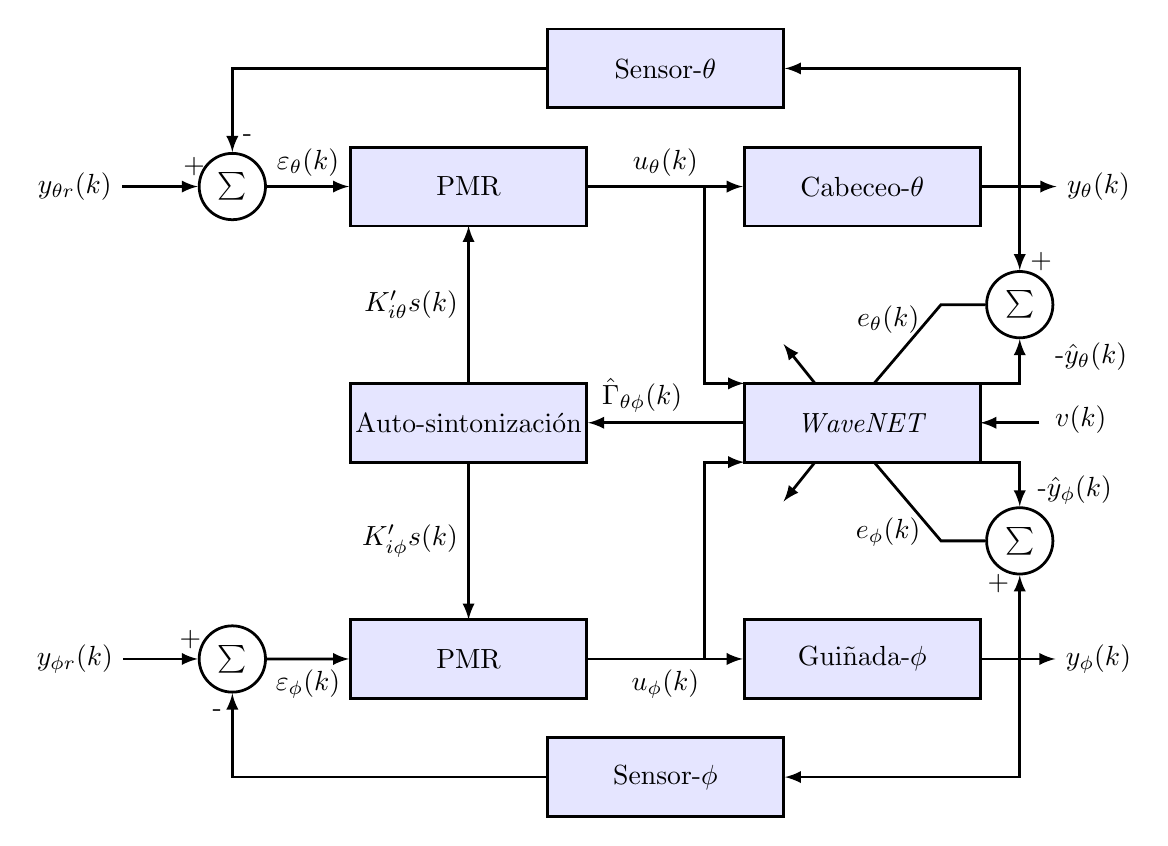
\begin{tikzpicture}[node distance = 5cm, auto, >=latex, line width = 1pt]
    \tikzstyle{block} = [draw, fill = blue!10, shape = rectangle, inner sep = 1pt, minimum height = 1cm, minimum width = 3cm]
    \tikzstyle{sum} = [draw, shape = circle, minimum size = 1em]

    \node[sum] (begin) at (0,0) {$\sum$};
    \node[] (start) [left of = begin, node distance = 2cm] {$y_{\theta r}(k)$};
    \node[block] (control) [right of = begin, node distance = 3cm] {PMR};
    \node[block] (process) [right of = control] {Cabeceo-$\theta$};
    \node[] (end) [right of = process, node distance = 3cm] {$y_{\theta}(k)$};
    \node[block] (gains) [below of = control, node distance = 3cm] {Auto-sintonización };
    \node[block] (rna) [below of = process, node distance = 3cm] {\textit{WaveNET}};
    \node[sum] (sum) at (10,-1.5) {$\sum$};
    \node[block] (sensor) at (5.5,1.5) {Sensor-$\theta$};
    
    \draw[->] (start) -- node[pos = 0.95] {+} (begin);
    \draw[->] (begin) -- node[pos = 0.50] {$\varepsilon_{\theta}(k)$} (control);
    \draw[->] (control) -- node {$u_{\theta}(k)$} (process);
        
    \draw[->] (3,-2.5) -- node {$K'_{i\theta}s(k)$} (3,-0.5);
    \draw[->] (10,0) -- node[pos = 0.9] {+} (sum);
    \draw[->] (9.25,-2.5) -| node[pos = 0.80, xshift = 1.5cm] {-$\hat{y}_{\theta}(k)$} (sum);
    \draw[->] (6.00,0) |- (6.5,-2.5);
    \draw[->] (10.25,-3) -- node[xshift = 0.90cm, yshift = 0.35cm]{$v(k)$} (9.5,-3);
    \draw[- ] (sum) -- (9,-1.5) -- node[pos = 0.5, above, xshift = -7pt]
        {$e_{\theta}(k)$} (8.15,-2.5);
    \draw[->] (7.4,-3.5) -- (7,-4);
    \draw[->] (10,0) |- (sensor);
    \draw[->] (sensor) -| node[pos = 0.9] {-} (begin);
    \draw[->] (process) -- (end);
    \draw[->] (rna) -- node[pos = 0.65, above] {$\hat{\Gamma}_{\theta\phi}(k)$} (gains);
    
    \node[sum] (begin2) at (0,-6) {\tiny $\sum$};
    \node[] (start2) [left of = begin2, node distance = 2cm] {$y_{\phi r}(k)$};
    \node[block] (control2) [below of = gains, node distance = 3cm] {PMR};
    \node[block] (process2) [below of = rna, node distance = 3cm] {\centering Guiñada-$\phi$};
    \node[] (end2) [right of = process2, node distance = 3cm] {$y_{\phi}(k)$};
    \node[block] (sensor2) at (5.5,-7.5) {Sensor-$\phi$};
    \node[sum] (sum2) at (10,-4.5) {$\sum$};
    
    \draw[<-] (3,-5.5) -- node {$K'_{i\phi}s(k)$} (3,-3.5);
    \draw[->] (start2) -- node[pos = 0.90] {+} (begin2);
    \draw[->] (begin2) -- node[pos = 0.50, below] {$\varepsilon_{\phi}(k)$} (control2);
    \draw[->] (control2) -- node[below] {$u_{\phi}(k)$} (process2);
    \draw[->] (6,-6) |- (6.5,-3.5);
    \draw[->] (10,-6) -- node[pos = 0.90] {+} (sum2);
    \draw[->] (9.25,-3.5) -| node[pos = 0.80, xshift = 0.7cm, below, yshift = 0.3cm] {-$\hat{y}_{\phi}(k)$} (sum2);
    \draw[->] (10,-6) |- (sensor2);
    \draw[->] (sensor2) -| node[pos = 0.90] {-} (begin2);
    \draw[->] (process2) -- (end2);
    
    \draw[- ] (sum2) -- (9,-4.5) -- node[pos = 0.5, above, xshift = -7pt, yshift = -0.7cm] {$e_{\phi}(k)$} (8.15,-3.5);
    \draw[->] (7.4,-2.5) -- (7,-2);
\end{tikzpicture}}
        \caption[Diagrama de bloques de los controladores PMR.]{Diagrama de bloques de los controladores proporcionales multiresolución.}
        \label{fig:schematicControlPMR}
    \end{figure}
        
     En palabras de \citeauthor{VegaNavarrete2013}, la señal de error se descompone en señales a diferentes niveles, la cuales se escalan con sus respectivas ganancias y al ser sumadas se obtiene la señal de control, que está expresada por \cite[p. 43]{VegaNavarrete2013} la siguiente ecuación
    \begin{equation}
        u(k) = \sum\limits_{i=1}^{N+1} K_i \varepsilon_i(k)
    \end{equation}
    \begin{eqexpl}
        \item{$N$} indica el nivel de resolución, 
        \item{$\varepsilon_i$} es la señal de error de la $i$-ésima escala, y
        \item{$K_i$} representa la ganancia para cada $i$-ésimo componente.
    \end{eqexpl}
        
        % Si se toma como ejemplo el control \acrshort{pid} discreto y recordando la \cref{equa:getsignal.vi} que proporciona su señal de control,
        
    Se puede indicar la nueva expresión que utilice el enfoque de multiresolución, es decir
    \begin{equation}
        u_{k+1} = u_{k} + \sum\limits_{i=1}^{3} K_i \varepsilon_{k(i)}
    \end{equation}
    \begin{eqexpl}
        \item{$k$}específica la época, y
        \item{$\sum$}se limita a tres, pues es la cantidad de componentes en el contraloador PID.
    \end{eqexpl}
        
    Como ya se dijo antes, la configuración del control PMR tiene la característica de emplear dos o más parámetros que dependen del nivel de resolución aplicada a la señal de error; la \cref{fig:structurePMR} muestra el diagrama empleado, mientras que el bloque de descomposición se ilustra en la \cref{fig:structure3levelsDescomp}.

    \begin{figure}[H]
        \centering
        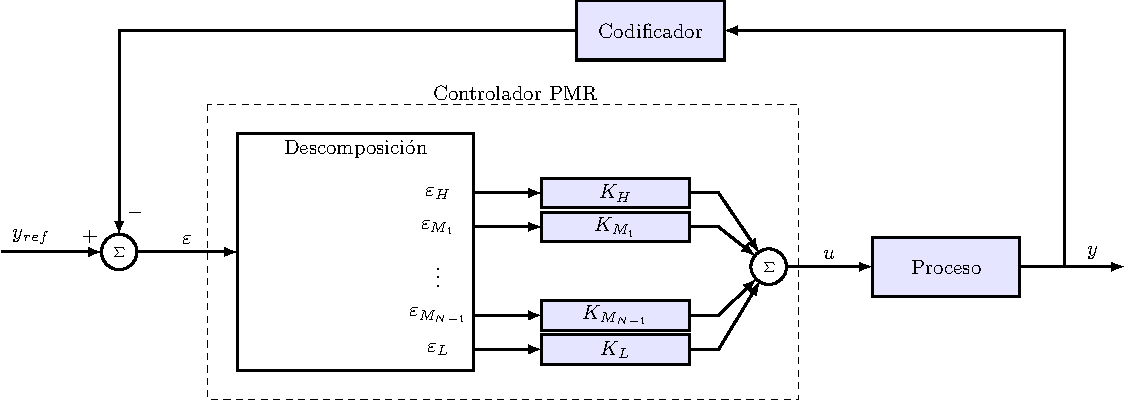
\includegraphics[width = \textwidth]{graphics/pmr/Block PMR Structure.pdf}
        \caption[Diagrama del controlador PMR en lazo cerrado.]{Diagrama del controlador PMR en lazo cerrado \cite[p. 48]{VegaNavarrete2013}.}
        \label{fig:structurePMR}
    \end{figure}
        
    \begin{figure}[H]
        \centering
        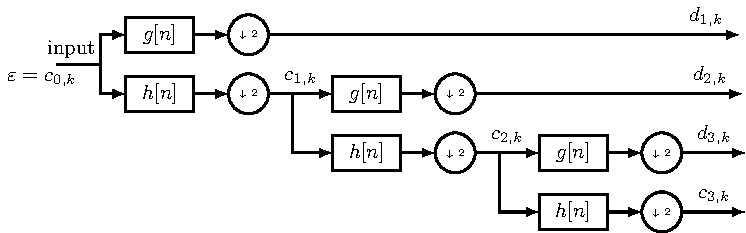
\includegraphics[width = 0.8\textwidth]{graphics/pmr/Filter Descomp 3 Levels.pdf}\\ \vspace*{0.5em}
        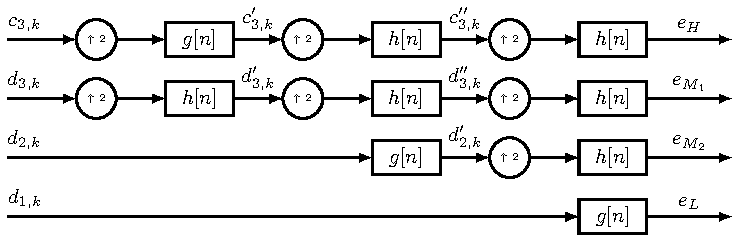
\includegraphics[width = 0.8\textwidth]{graphics/pmr/Filter Sint 3 Levels.pdf}
        \caption[Diagrama de análisis de tres niveles.]{Diagrama de descomposición y síntesis de tres niveles \cite[p. 47]{VegaNavarrete2013}.}
        \label{fig:structure3levelsDescomp}
    \end{figure}
        
     La expresión general para escalar los componentes es
    \begin{align}
        u &= K_{H}\varepsilon_{H} + K_{M_1}\varepsilon_{M_1} + \cdots + K_{i}\varepsilon_{i} + \cdots + K_{L}\varepsilon_{L}
    \end{align}
    que expresándola en su forma matricial se tiene
    \begin{align}
        u &= \mathbf{K}\odot\mathbf{E_m},\,\text{siendo} \\
        \mathbf{K} &= 
            \begin{bmatrix}
                K_{H} & K_{M_1} & \cdots & K_{i} & \cdots & K_{L}
            \end{bmatrix},\,\text{y}\\
        \mathbf{E_m} &= 
            \begin{bmatrix}
                \varepsilon_{H} & \varepsilon_{M_1} & \cdots & \varepsilon_{i} & \cdots & \varepsilon_{L}
            \end{bmatrix}.
    \end{align}
        
    Finalmente, \citeauthor{VegaNavarrete2013} presenta las reglas de sintonización automática, las cuales están implícitas en las leyes del control anterior, por lo tanto se tiene
    \begin{align}
        K_{H}[k+1] &= (K_{H}[k]T + \mu_{H} \hat{\Gamma} (\varepsilon_H[k] - \varepsilon_H[k]))/T \\
        K_{M_1}[k+1] &= (K_{M_1}[k-1]T + \mu_{M_1} \hat{\Gamma} (\varepsilon_{M_1}[k] - \varepsilon_{M_1}[k-1]))/T \\
        &\vdots \\
        K_{M_{N-1}}[k+1] &= (K_{M_{N-1}}[k-1]T + \mu_{M_{N-1}} \hat{\Gamma} (\varepsilon_{M_{N-1}}[k] - \varepsilon_{M_{N-1}}[k-1]))/T \\
        K_{L}[k+1] &= (K_{L}[k-1]T + \mu_{L} \hat{\Gamma} (\varepsilon_L[k] - \varepsilon_L[k-1]))/T
    \end{align}
    donde
    \begin{align}
        \Gamma[k] &= \sum\limits_{i=0}^{M} c_i z[k-i]u[k]
    \end{align}
    y las $\mu$ se tratan de la taza de actualización o aprendizaje del controlador.

        % Los resultados obtenidos en la \cref{sec:ident_fOut} fueron tomados como base, pues la configuración encontrada para la \textit{wavenet} ya cuenta con el entrenamiento, entonces sólo fue necesario realizar la operación dentro de línea para hallar los parámetros del nuevo controlador.
\section{Identificación fuera línea}\label{sec:PMR_outline}
        
\section{Identificación en línea}\label{sec:PMR_online}